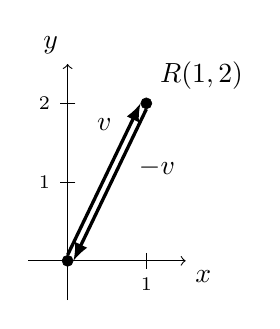
\begin{tikzpicture}[
	point/.style={circle,draw,very thin,fill,inner sep=0pt,minimum size=4pt},
	vector/.style={-latex},
]
  \draw[->] (-0.5,0) to (1.5,0) node[below right] {$x$};
  \draw[->] (0,-0.5) to (0,2.5) node[above left] {$y$};

	\foreach \x in {1} {
		\draw (\x,0.1) to (\x,-0.1) node[below] {$\scriptstyle \x$};
	}
	\foreach \y in {1,2} {
		\draw (0.1,\y) to (-0.1,\y) node[left] {$\scriptstyle \y$};
	}

	\node[point] at (0,0) (o) {};
	\node[point] at (1,2) (r) [label=above right:{$R(1,2)$}] {};
	\draw[vector,very thick] (o.north) to node[above left,near end] {$\uvec{v}$} (r.west);
	\draw[vector,very thick] (r.south) to node[below right, near start] {$-\uvec{v}$} (o.east);

\end{tikzpicture}
